% erstewoche/checkliste.tex

Die ersten Wochen an der Uni sind erfahrungsgemäß die schlimmsten: Wir haben euch hier die wichtigsten Punkte zusammengestellt, um die ihr euch in den ersten Tagen bzw. Wochen kümmern solltet. Man findet sich im großen Chaos Universität ziemlich schnell zurecht -- Don't panic!
  
  \begin{enumerate}[label=$\bigcirc$]
  	
  	\item \textbf{FAQ} \\
		Eine Übersicht der häufigsten Fragen und deren Antworten findet ihr unter \url{https://uni-tuebingen.de/fakultaeten/mathematisch-naturwissenschaftliche-fakultaet/fachbereiche/informatik/studium/studiengaenge/informatik/faq/}.
	\item \textbf{Zum Übungsbetrieb anmelden} \\
	  	Oft muss man, um zur Klausur einer Veranstaltung zugelassen zu werden, eine bestimmte Anzahl an Punkten in den Übungsblättern erreichen. Damit ihr die Übungen machen könnt, müsst ihr euch in der Veranstaltung dazu anmelden. Wie das geht, erfahrt ihr in den ersten Vorlesungen (oft sogar direkt in der ersten Vorlesung, also nicht verpassen!).
  	\item \textbf{Übungspartner suchen} \\
	  	Übungsblätter im Alleingang zu machen ist zwar möglich, aber schwierig. Sucht euch daher am besten gleich am Anfang pro Veranstaltung mit Übungsbetrieb einen Übungspartner, mit dem ihr die Blätter abgeben könnt.
  	\item \textbf{WLAN-Zugang mit eduroam einrichten}\\
	  	Mit euren ZDV-Login-Daten (i.d.R. \texttt{zxabc12@uni-tuebingen.de} und dem ZDV-Passwort) könnt ihr uni-weit kostenlos per WLAN ins Internet. \textbf{Wichtig:} Bindet ein Zertifikat ein! Eine ausführliche Anleitung hierzu findet ihr im Kapitel Infrastruktur.
  	\item \textbf{Erstwohnsitz in Tübingen anmelden} \\
	  	Sofern ihr mit dem Studienbeginn neu nach Tübingen gezogen seid, solltet ihr euch innerhalb von zwei Wochen bei der Stadtverwaltung anmelden. Hierfür benötigt ihr eine Kopie des Mietvertrages und die Wohnungsgeberbescheinigung. Es ist ratsam, seinen Erstwohnsitz in Tübingen anzumelden und z.B. das elterliche Wohnhaus als Zweitwohnsitz anzugeben, da Tübingen eine Zweitwohnsitzsteuer erhebt.
	\item \textbf{Postadresse im CAMPUS aktualisieren}\\
		Die ZV der Uni schickt euch jedes Semester nachdem ihr euch erfolgreich rückgemeldet habt euer neues Datenkontrollblatt zu, in dem ihr u.A. die Bescheinigung für das Semesterticket findet. Damit dieser Brief nicht immer an die falsche Adresse geht, solltet ihr im CAMPUS-System eure Adresse aktualisieren.
	\item \textbf{Rundfunkbeitrag} \\
		Diesen Brief bekommt ihr normalerweise, sobald ihr euch nach Tübingen umgemeldet habt. Die Rundfunkgebühren müssen nur von einer Person pro Haushalt bezahlt werden, fragt also eure Mitbewohner oder Vermieter, ob schon bezahlt wird! Wenn ihr BaföG bezieht, könnt ihr euch u.U. vom Rundfunkbeitrag befreien lassen. Mehr Infos hierzu auch unter \url{https://www.rundfunkbeitrag.de/}.
  \end{enumerate}

\begin{center}
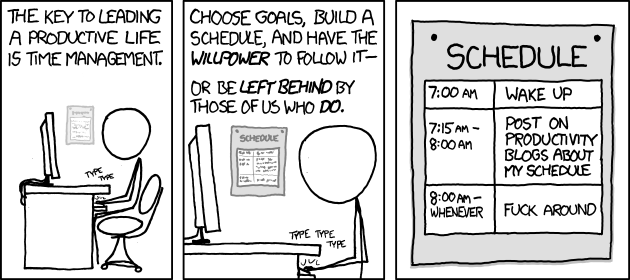
\includegraphics[width=0.5\hsize]{info/xkcd/time_management.png}
\end{center}

